\documentclass{article}
\usepackage{graphicx}
\usepackage{hyperref}
\usepackage{amsmath}
\usepackage{times}
\usepackage{enumerate}
\usepackage{cite}
\usepackage{placeins}

\textwidth=6.2in
\textheight=8.5in
%\parskip=.3cm
\oddsidemargin=.1in
\evensidemargin=.1in
\headheight=-.3in


%------------------------------------------------------------
% newcommand
%------------------------------------------------------------
\newcommand{\scscst}{\scriptscriptstyle}
\newcommand{\scst}{\scriptstyle}
\newcommand{\Robject}[1]{{\texttt{#1}}}
\newcommand{\Rfunction}[1]{{\texttt{#1}}}
\newcommand{\Rclass}[1]{\textit{#1}}
\newcommand{\Rpackage}[1]{\textit{#1}}
\newcommand{\Rexpression}[1]{\texttt{#1}}
\newcommand{\Rmethod}[1]{{\texttt{#1}}}
\newcommand{\Rfunarg}[1]{{\texttt{#1}}}

\usepackage{Sweave}
\begin{document}
\Sconcordance{concordance:FinalPaper.tex:FinalPaper.Rnw:%
1 30 1 1 0 43 1 1 6 1 2 35 1 1 7 12 0 1 2 4 1 2 2 6 1 1 3 1 2 8 1 1 4 %
14 0 1 2 4 1 1 2 12 0 1 2 26 1 1 9 38 0 1 2 4 1 1 4 38 0 1 2 4 1 1 35 1 %
2 1 3 1 2 1 3 1 2 1 4 1 2 6 1 1 5 37 0 1 2 6 1 2 2 4 1 2 2 12 1 1 2 1 0 %
1 2 1 0 1 4 3 0 1 2 1 0 1 3 2 0 1 2 1 0 1 2 24 0 1 2 4 1 1 3 2 0 1 3 2 %
0 1 2 1 0 1 4 69 0 1 2 4 1 1 6 2 2 1 12 6 1 1 5 36 0 1 2 8 1 1 8 7 0 1 %
1 1 8 7 0 1 4 3 0 1 2 7 0 1 2 6 1 1 8 7 0 1 1 1 8 7 0 1 4 3 0 1 2 7 0 1 %
2 4 1 1 2 33 0 1 2 4 1 1 10 10 0 1 8 1 3 4 1 1 2 1 0 1 2 1 0 1 2 38 0 1 %
2 67 1}


%------------------------------------------------------------
\title{Regression Analysis of Higher Education Outcomes}
%------------------------------------------------------------
\author{Gilbert Watson, David Wasser, and Paul Biedlingmaier}
\date{Thursday, December 19th, 2013}





\maketitle
\tableofcontents

%-------------------------------------------
\section{Introduction}
%-------------------------------------------

Higher education is a big business. College students, their parents, student loan companies, and the federal government dump huge amounts of money into the endeavor every year. Given the large amounts of money involved, many may wonder what post-secondary institutions are doing the best per dollar spent in terms of achieving education outcomes? While this paper doesn't seek to examine that question in its entirety, it does seek to examine a small component - education outcomes as measured by graduation rates. High graduation rates are indicative high achieving institution. What types of institutional characteristics cause there to be high graduation rates? After controlling for various characteristics, is there a relationship between tuition costs and a school with a higher graduation rate? These are important questions that are very pertinent to soon to be college students. If they can expect to receive a better education (or at least a more expedient one) just by paying more (all other things being equal) then that would be a good piece of information to know.

This paper seeks to examine the relationship between graduation rates and other post-secondary institutional factors through a variety of means. Using a widely available government data set, one-way, two-way, and regression analyses are conducted, all in an attempt to understand the drivers behind graduation rates.

%-------------------------------------------
\section{Methods and Materials: The Data}
%-------------------------------------------

\subsection{Raw Data}
Data on five year graduate rates, tuition and fees, and other post-secondary institutional characteristics are available through the US Department of Education's National Center for Education Statistics (NCES) \footnote{http://nces.ed.gov/datatools/}. For this study, we chose to only consider data for those institutions that possess the following characteristics:

\begin{enumerate}[a)]
\item{} Title IV participating
\item{} US only
\item{} Carnegie Foundation ranking in a research, doctoral, or baccalaureate category
\item{} The institution has at least some full-time undergraduates
\item{} The institution has at least one program that is not offered through distance education
\item{} No for-profit institutions, only public and not-for-profit
\end{enumerate}

The survey that collects this data is administered yearly, but for this study, we chose to only consider the cross section available from the 2010 survey. We do not intend to examine the time dynamics of institutional characteristics.

The original data set contains 1499 observational units and 320 variables. Variables contain data on characteristics such as admission rates, admission yields, tuition and other costs, student body demographics, graduation rates, averages and percentages of students receiving various types of aid, pay rates for different types of university faculty, and various institutional financials on a per faculty basis. In particular, this paper seeks to examine the relationship between five year undergraduate graduation rates and other variables in the data set. Five year graduate rates are a proxy for educational quality in that they measure the intended outcome of higher education - earning a degree. One would imagine that institutions that deliver high educational outcomes, like a high graduation rate for its students would potentially cost more. Is this the case? Is there a relationship between graduation rates and the type of institution whether that institution be public or private? Controlling for the selectivity of an institution, which likely has a relationship with graduation rates itself, is there a relationship between how much a person pays for college and the college's ability to produce graduates? These are the questions this paper seeks to answer. To begin, let's take a look at a motivating scatter plot. 

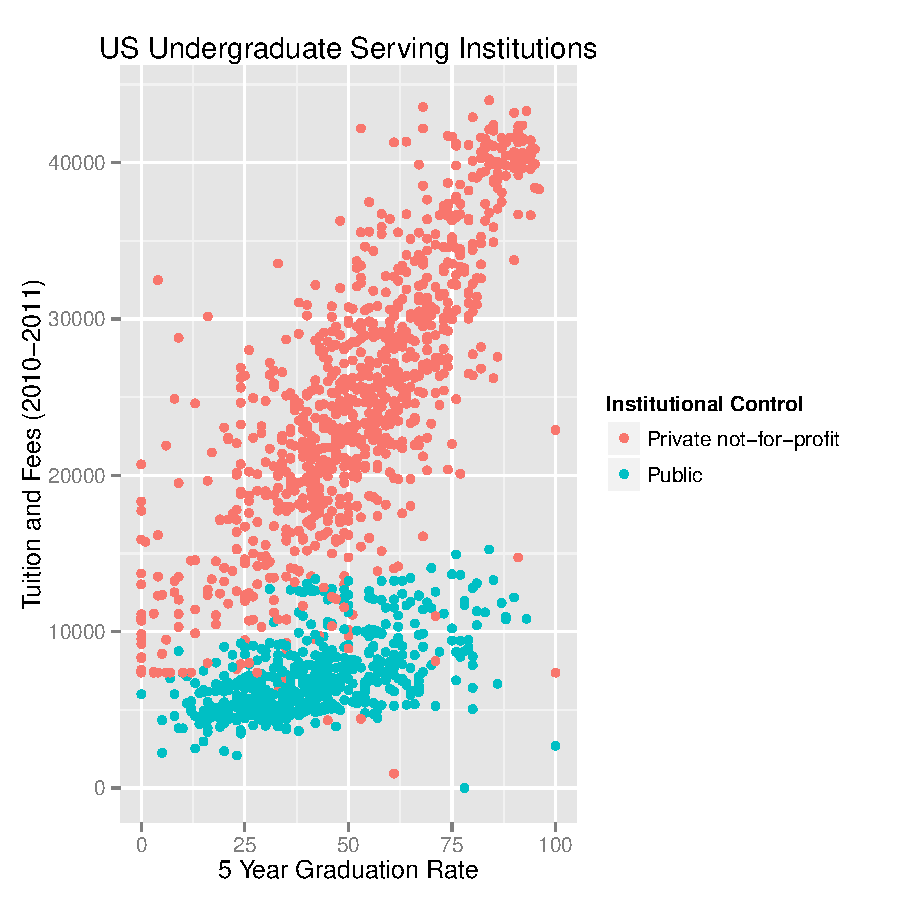
\includegraphics{Fig-sourceanalysis1}

A quick examination of this plot shows that there is in fact a relationship between graduation rates and cost. A scatter plot of five year graduation rates and tuition and fees shows the existence of a strong relationship. It also shows a relationship that is bifurcated between private and public institutions. This isn't surprising. Public school tuition is largely subsidized, so we would expect an interaction between costs and the public, private status of the institution. We will begin with an ANOVA analysis of this relationship, but we are not concerned with this relationship alone. After conducting both one-way and two-way ANOVA, this paper will seek to generate a regression model for graduation rates using the best predictors from the data set. Just because we see the existence of a strong relationship between costs, public/private status, and graduation rates does not mean that there are no other underlying and significant relationships of interest.

\FloatBarrier

While the data relating to the ANOVA analysis is largely clean and complete in the database, more extensive cleaning measure were taken to conduct regression analysis. A quick discussion of the steps taken to clean the data should executed before we jump into analysis.

\subsection{Data Cleaning}

Several steps were taken to clean the data prior to analysis. A full accounting of the steps taken is in the source code for this document, which will be made available on Github \footnote{https://github.com/GilbertWatson/LinearRegressionProject}. A list of the high points which do concern the analysis follows:

\begin{enumerate}[a)]
\item{} Institutional identification variables were removed.
\item{} A small collection of variables concerning a particular cohort of students measured by NCES was removed.
\item{} The small differences between FASB and GASB financial reporting methods for educational institutions are ignored and those variables are merged. These largely comprise per full-time equivalent institutional finance variables.
\item{} In-state and out-of-state cost variables are merged for private institutions where they have no applicability
\item{} Admission rates for institutions that only serve one gender were adjusted to zero for the appropriate gender. Additionally, a categorical variable indicating whether an institution serves males, females, or both was generated.
\item{} One pair of variables that partitioned the data were removed to eliminate the possibility of linear dependence between columns. For example, percentage of students enrolled in non-degree programs was removed as a variable in the presence of full-time and part-time enrollment because all three would perfectly partition the total enrollment variable.
\item{} Several variable transformations were preformed before analysis to eliminate obvious sources of co-linearity. For example, the percentage of enrollment comprised of undergrads was generated to account for the fact that undergraduate enrollment and total enrollment are highly correlated. None of the original variables were removed and are still taken into consideration as predictors, but the transformations made seemed like obvious normalizations.
\item{} Variables that are missing for over 100 observations are removed from the data set. This eliminates variables like the revenue from state appropriations since most private schools do not receive state appropriations.
\end{enumerate}

%-------------------------------------------
\section{Methods and Materials: ANOVA Analysis}
%-------------------------------------------

Using the raw, uncleaned data set, we conducted an initial set of ANOVA analyses.

\subsection{One-Way ANOVA}

We first conduct an analysis of variance to explore the relationship between the institution’s 5-year graduation rate and its status as a public or private not-for-profit institution (Table 1). Our initial motivating scatter plot suggests that there may be differences in graduation rates achieved by these two types of institutions, but it is hard to say for sure. While there is a clear split between the two groups in terms of tuition and fees, there a quite a few of both types for each level of graduation rate. It is easy to calculate that the mean graduation rate for public institutions is $41.81$ and $52.72$ for private institutions, but is there a true, statistical difference between the two groups?

$$ H_0\text{: No Difference Between Groups} $$
$$ H_a\text{: Difference Between Groups} $$
$$ \text{If }F^* > F(0.99,2,1465)\text{ Reject }H_0 $$

% latex table generated in R 3.0.2 by xtable 1.7-1 package
% Thu Dec 19 11:05:31 2013
\begin{table}[ht]
\centering
\begin{tabular}{rrrrr}
  \hline
 & Estimate & Std. Error & t value & Pr($>$$|$t$|$) \\ 
  \hline
HD2011.Control.of.institutionPrivate not-for-profit & 52.7199 & 0.6684 & 78.88 & 0.0000 \\ 
  HD2011.Control.of.institutionPublic & 41.8095 & 0.8681 & 48.16 & 0.0000 \\ 
   \hline
\end{tabular}
\caption{ANOVA: Grad Rates vs. Public/Private} 
\end{table}
\FloatBarrier

From the table above, we can see that we should reject $H_0$. Graduation rates do differ between public and private institutions. We should note make a quick note that this ANOVA model doesn't quite meet the assumptions required. For one, there is evidence of unequal variances between groups as evidenced by a p-value for the Breusch-Pagan test of $3.53260243945052e-06$. Secondly, the residuals, while distributed symmetrically, are clearly not distributed normally when viewing a QQ plot. We will attempt to use a more sophisticated regression model to deal with these problems later.

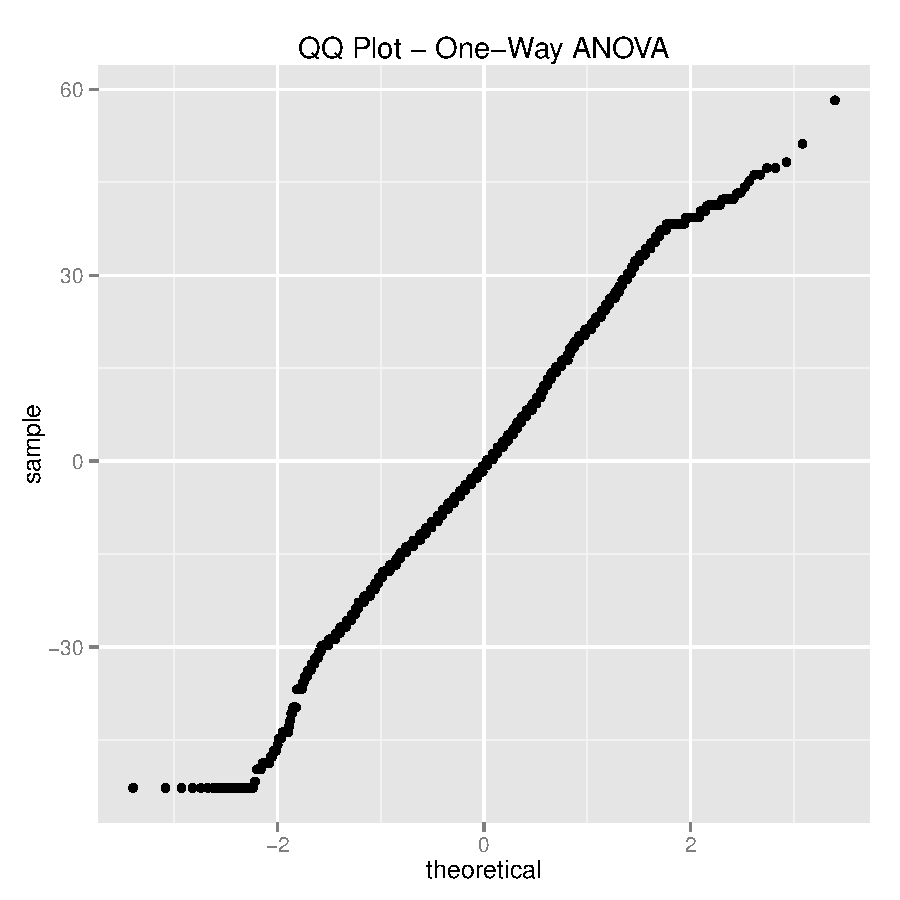
\includegraphics{Fig-anotherdamnqq}

\FloatBarrier

\subsection{Two-Way ANOVA}

Despite the results of the one-way ANOVA analysis, it is clear from our motivating scatter plot that there are additional factors at play. Even though public schools have a lower five year graduation rate on average, there still are public schools that perform at similar levels to private institutions. It is possible that selectivity has a role to play in this. Perhaps the most selective public schools produce graduates by the five year mark at the same rate as private institutions. A visual representation of this relationship is not quite as clean as our motivating graphic.

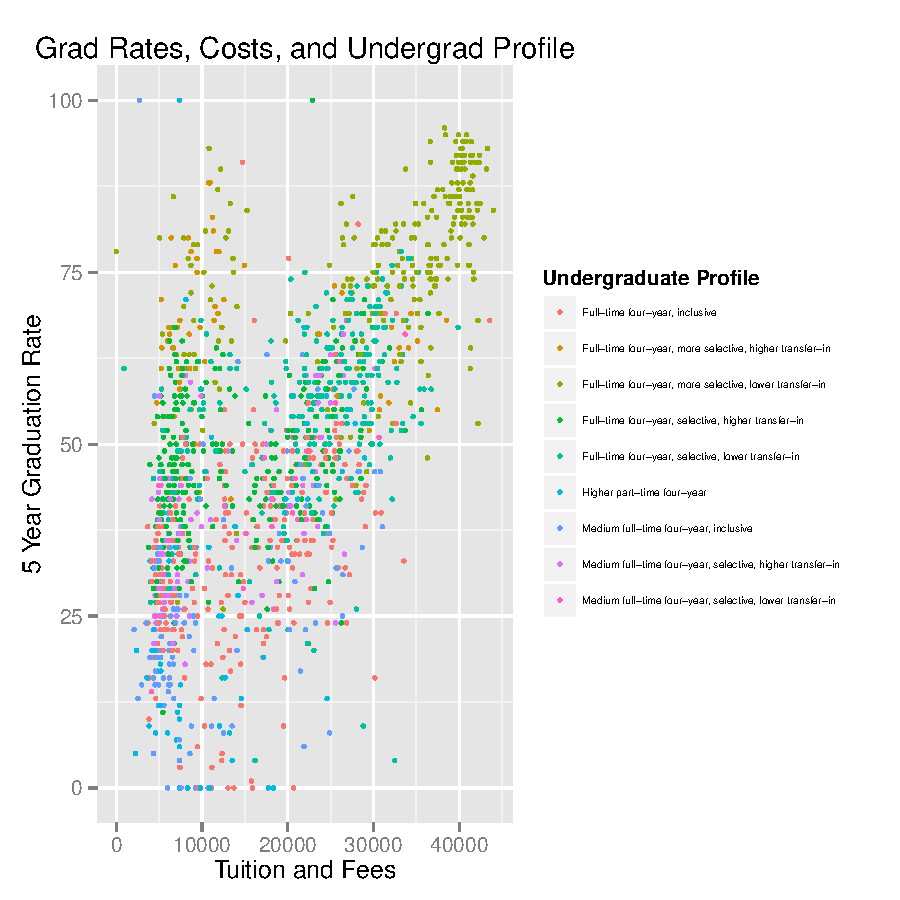
\includegraphics{Fig-anovaplot}

\FloatBarrier

A way to test for this is to conduct two-way ANOVA analysis and conduct an F-test for the significance of the within-groups effect using the Carnegie Classification for an institution's undergraduate program's selectivity as the second tabular dimension. This variable partitions the institutions into various levels of selectivity and programs types and will be a good proxy for the effect we are trying to understand. 

$$ H_0\text{: No Difference Within Groups} $$
$$ H_a\text{: Difference Within Groups} $$
$$ \text{If }F^* > F(0.99,8,1449)\text{ Reject }H_0 $$

% latex table generated in R 3.0.2 by xtable 1.7-1 package
% Thu Dec 19 11:05:32 2013
\begin{table}[ht]
\centering
\begin{tabular}{lrrrrr}
  \hline
 & Df & Sum Sq & Mean Sq & F value & Pr($>$F) \\ 
  \hline
HD2011.Control.of.institution & 2 & 3514241.08 & 1757120.54 & 10109.19 & 0.0000 \\ 
  HD2011.Carnegie.Classification.2010..Undergraduate.Profile & 8 & 345942.11 & 43242.76 & 248.79 & 0.0000 \\ 
  HD2011.Control.of.institution:HD2011.Carnegie.Classification.2010..Undergraduate.Profile & 8 & 4985.13 & 623.14 & 3.59 & 0.0004 \\ 
  Residuals & 1449 & 251856.68 & 173.81 &  &  \\ 
   \hline
\end{tabular}
\caption{Two-Way ANOVA: Grad Rates vs. Inst.Sector and Inst. Control} 
\end{table}
\FloatBarrier

It is clear from the table above that we do reject $H_0$ and conclude that even within groups of similar selectivity and type there are differences between public and private institutions' graduation rates. A table of the reduction in residual sum of squares and the significance of the addition of selectivity type variables follows.

% latex table generated in R 3.0.2 by xtable 1.7-1 package
% Thu Dec 19 11:05:32 2013
\begin{table}[ht]
\centering
\begin{tabular}{lrrrrrr}
  \hline
 & Res.Df & RSS & Df & Sum of Sq & F & Pr($>$F) \\ 
  \hline
1 & 1465 & 602783.92 &  &  &  &  \\ 
  2 & 1449 & 251856.68 & 16 & 350927.24 & 126.19 & 0.0000 \\ 
   \hline
\end{tabular}
\caption{ESS Table: Addition of Inst. Sector} 
\end{table}
\FloatBarrier

We must again note that this model suffers from the same issues associated with the one-way ANOVA analysis (a p-value for the Breusch-Pagan statistic of $2.5548088759262e-14$ and a similar profile QQ plot). A more sophisticated model is necessary to deal with these issues and better explain the variation in graduation rates among institutions. A model that includes more predictors may alleviate some of the issues underlying the ANOVA analysis. A more sophisticated model will also reveal deeper relationships at play that just those between institutional classification and graduation rates.

%-------------------------------------------
\section{Methods and Materials:  Regression Analysis of 5 Year Graduation Rates}
%-------------------------------------------

\subsection{Dimensionality Reduction}

319 potential predictors is a daunting number of variables to deal with. For the purposes of regression analysis, and without any qualitative understanding of the drivers behind graduation rates and tuition and fees other than those explored by ANOVA analysis, an automated variable selection method was used to reduce the data set to a manageable number of predictors. This step was used to generate an initial first order regression model for five year graduation rates. As it was a rather extensive effort, and as it greatly influenced our analysis, a discussion of the method used is given its own section. The following steps were taken to reduce the data set to a size manageable for more detailed modeling.

\begin{enumerate}[1)]
\item{} Variables closely related to the response were removed from the data set. For example, 4 and 6 year graduation rates were removed since they are so closely related to the 5 year graduation rate.
\item{} The full model with all remaining candidate predictors is estimated.
\item{} Using the full model, forward, backward, and sequential automated variable selection algorithms are used to search for the best reduced model. Each method is was allowed to pick a set of up to 50 predictors which optimized model BIC. The union of these predictors is passed to the next step.
\item{} All but those predictors proposed by the previous step are removed from the data set. A full model with those predictors remaining is estimated. Again, the three methods of automated variable selection choose the best model available to the algorithm using BIC as a criterion. Each is allowed to consider models of up to 20 predictors. The union of these predictors is passed to the next step.
\item{} Only those predictors selected by the previous step are retained in the data set. An efficient branch-and-bound algorithm is used to search the remaining predictors for the best model. The criterion doesn't matter since the search is exhaustive. The predictors selected by this step are used as the initial step in modeling.
\end{enumerate}

The reason for using multiple stages of automated variable selection is that exhaustive search for the best model using just first order terms would be very computationally intensive using the full set of predictors. This method gives us a manageable number of predictors to begin model refinement. Even graphical search for potential predictors would have been difficult with so many potential variables. Consider that there would have been over fifty thousand paired scatter plots to consider. This method effectively delivers a working data set containing only those predictors that are most explanatory of five year graduation rates. Most importantly, it delivers a smaller data set, giving us a manageable place to start model refinement.

\subsection{Initial Model}

After the initial data reduction effort described above, an initial model for five year undergraduate graduation rates results. The table below gives the summary statistics for the data set underlying the model:

% latex table generated in R 3.0.2 by xtable 1.7-1 package
% Thu Dec 19 11:05:33 2013
\begin{table}[ht]
\centering
\begin{tabular}{rrrrr}
  \hline
 & Min & Median & Mean & Max \\ 
  \hline
Five.Year.Bachelors.Graduation.Rate & 0.00 & 49.00 & 49.69 & 100.00 \\ 
  Tuition.Fees.2009.2010 & 876.00 & 18200.00 & 17877.57 & 42335.00 \\ 
  Tuition.Fees.2010.2011 & 910.00 & 19015.00 & 18741.26 & 43990.00 \\ 
  Mid.East & 0.00 & 0.00 & 0.19 & 1.00 \\ 
  Distant.Degree.of.Urbanization & 0.00 & 0.00 & 0.03 & 1.00 \\ 
  UgradProfile.FullTime.MoreSelective.HighTransfer & 0.00 & 0.00 & 0.05 & 1.00 \\ 
  UgradProfile.FullTime.MoreSelective.LowTransfer & 0.00 & 0.00 & 0.18 & 1.00 \\ 
  UgradProfile.FullTime.Selective.HighTransfer & 0.00 & 0.00 & 0.20 & 1.00 \\ 
  UgradProfile.FullTime.Selective.LowTransfer & 0.00 & 0.00 & 0.19 & 1.00 \\ 
  UgradProfile.Medium.FullTime.Selective.Inclusive & 0.00 & 0.00 & 0.08 & 1.00 \\ 
  SizeSetting.Large.FourYear.NotResidential & 0.00 & 0.00 & 0.08 & 1.00 \\ 
  SizeSetting.Medium.FourYear.NotResidential & 0.00 & 0.00 & 0.08 & 1.00 \\ 
  SizeSetting.Small.FourYear.NotResidential & 0.00 & 0.00 & 0.06 & 1.00 \\ 
  SizeSetting.Small.FourYear.Residential & 0.00 & 0.00 & 0.11 & 1.00 \\ 
  SizeSetting.VSmall.FourYear.NotResidential & 0.00 & 0.00 & 0.01 & 1.00 \\ 
  Undergraduate.Enrollment & 71.00 & 2752.00 & 5880.41 & 58404.00 \\ 
  First.Time.Certificate.Seeking.Ugrad.Enrollment & 10.00 & 559.00 & 1060.16 & 9254.00 \\ 
  First.Time.Full.Time.Certificate.Seeking.Ugrad.Enrollment & 6.00 & 548.00 & 1029.94 & 9082.00 \\ 
  Percent.Total.Enrollment.White & 0.00 & 68.00 & 62.05 & 97.00 \\ 
  Full.Time.Retention.Rate.2011 & 21.00 & 75.00 & 74.63 & 99.00 \\ 
  Bachelors.Degrees.Awarded & 8.00 & 511.00 & 1103.17 & 12194.00 \\ 
  Percent.First.Time.Full.Time.Ugrad.Pell.Grant.Recipients & 6.00 & 39.00 & 40.73 & 100.00 \\ 
  Investment.Return.As.Percent.Core.Revenue & -5.00 & 6.00 & 12.30 & 89.00 \\ 
  Endowment.Per.FTE.Enrollment & 11.00 & 9974.00 & 44175.56 & 2398707.00 \\ 
  Male.Female.Full.Time.Admission.Yeild.Difference & -48.00 & 2.00 & 1.95 & 40.00 \\ 
  Percent.First.Time.Transfer.Ugrad.Enrollment & 0.00 & 0.06 & 0.07 & 0.33 \\ 
  Assistant.Percentage.Full.Prof.Salary & -0.37 & -0.13 & -0.13 & 0.18 \\ 
  Percent.Average.Student.Loan.Of.Tuition.Ugrad & 0.06 & 0.40 & 0.60 & 2.59 \\ 
   \hline
\end{tabular}
\caption{Summary Statistics For Dataset (n = 1351)} 
\end{table}
\FloatBarrier

If we estimate a full model, using all of this truncated data set, we see the following estimates of coefficients and their individuals p-values.

% latex table generated in R 3.0.2 by xtable 1.7-1 package
% Thu Dec 19 11:05:33 2013
\begin{table}[ht]
\centering
\begin{tabular}{rrrrr}
  \hline
 & Estimate & Std. Error & t value & Pr($>$$|$t$|$) \\ 
  \hline
(Intercept) & -1.7389 & 3.4773 & -0.50 & 0.6171 \\ 
  Tuition.Fees.2009.2010 & 0.0009 & 0.0005 & 1.94 & 0.0532 \\ 
  Tuition.Fees.2010.2011 & -0.0006 & 0.0005 & -1.36 & 0.1730 \\ 
  Mid.East & 1.9509 & 0.5710 & 3.42 & 0.0007 \\ 
  Distant.Degree.of.Urbanization & -5.8324 & 1.3631 & -4.28 & 0.0000 \\ 
  UgradProfile.FullTime.MoreSelective.HighTransfer & 4.7225 & 1.2972 & 3.64 & 0.0003 \\ 
  UgradProfile.FullTime.MoreSelective.LowTransfer & 5.9283 & 1.0681 & 5.55 & 0.0000 \\ 
  UgradProfile.FullTime.Selective.HighTransfer & 2.1294 & 0.6975 & 3.05 & 0.0023 \\ 
  UgradProfile.FullTime.Selective.LowTransfer & 2.4710 & 0.7805 & 3.17 & 0.0016 \\ 
  UgradProfile.Medium.FullTime.Selective.Inclusive & -2.5668 & 0.8899 & -2.88 & 0.0040 \\ 
  SizeSetting.Large.FourYear.NotResidential & -6.1480 & 1.1380 & -5.40 & 0.0000 \\ 
  SizeSetting.Medium.FourYear.NotResidential & -6.4913 & 0.9431 & -6.88 & 0.0000 \\ 
  SizeSetting.Small.FourYear.NotResidential & -4.9056 & 0.9843 & -4.98 & 0.0000 \\ 
  SizeSetting.Small.FourYear.Residential & -2.8344 & 0.7578 & -3.74 & 0.0002 \\ 
  SizeSetting.VSmall.FourYear.NotResidential & -6.0641 & 1.8418 & -3.29 & 0.0010 \\ 
  Undergraduate.Enrollment & -0.0016 & 0.0002 & -8.19 & 0.0000 \\ 
  First.Time.Certificate.Seeking.Ugrad.Enrollment & 0.0105 & 0.0031 & 3.41 & 0.0007 \\ 
  First.Time.Full.Time.Certificate.Seeking.Ugrad.Enrollment & -0.0087 & 0.0029 & -2.98 & 0.0029 \\ 
  Percent.Total.Enrollment.White & 0.0713 & 0.0127 & 5.59 & 0.0000 \\ 
  Full.Time.Retention.Rate.2011 & 0.6332 & 0.0315 & 20.07 & 0.0000 \\ 
  Bachelors.Degrees.Awarded & 0.0069 & 0.0007 & 9.99 & 0.0000 \\ 
  Percent.First.Time.Full.Time.Ugrad.Pell.Grant.Recipients & -0.1298 & 0.0235 & -5.52 & 0.0000 \\ 
  Investment.Return.As.Percent.Core.Revenue & 0.0562 & 0.0224 & 2.51 & 0.0121 \\ 
  Endowment.Per.FTE.Enrollment & 0.0000 & 0.0000 & 3.22 & 0.0013 \\ 
  Male.Female.Full.Time.Admission.Yeild.Difference & -0.1236 & 0.0282 & -4.37 & 0.0000 \\ 
  Percent.First.Time.Transfer.Ugrad.Enrollment & -19.6618 & 7.2701 & -2.70 & 0.0069 \\ 
  Assistant.Percentage.Full.Prof.Salary & -11.7602 & 3.6215 & -3.25 & 0.0012 \\ 
  Percent.Average.Student.Loan.Of.Tuition.Ugrad & -2.9308 & 1.0626 & -2.76 & 0.0059 \\ 
   \hline
\end{tabular}
\caption{F = 289.7726 (n = 1351 on 1323 degrees of freedom)} 
\end{table}
\FloatBarrier

The first thing we should do is examine scatter plots of the five year graduation rate with other, non-binary variables in the reduced data set, just to get a sense of the relationships between the predictors and the five year graduation rate.

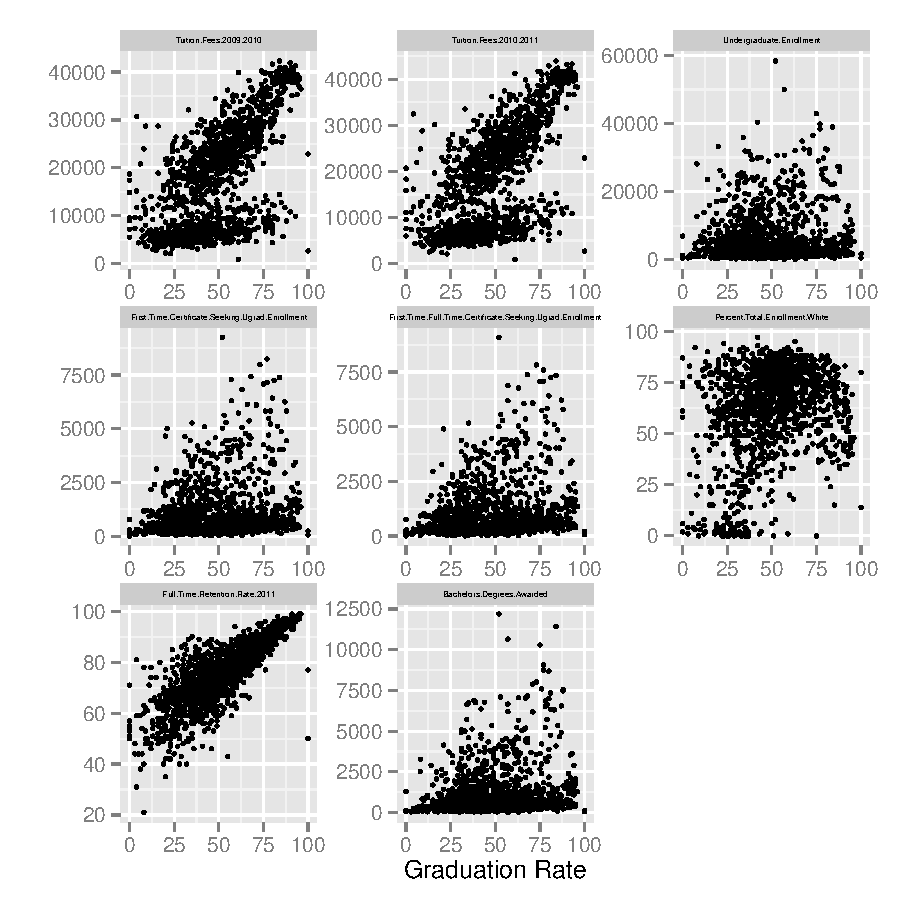
\includegraphics{Fig-pairs}

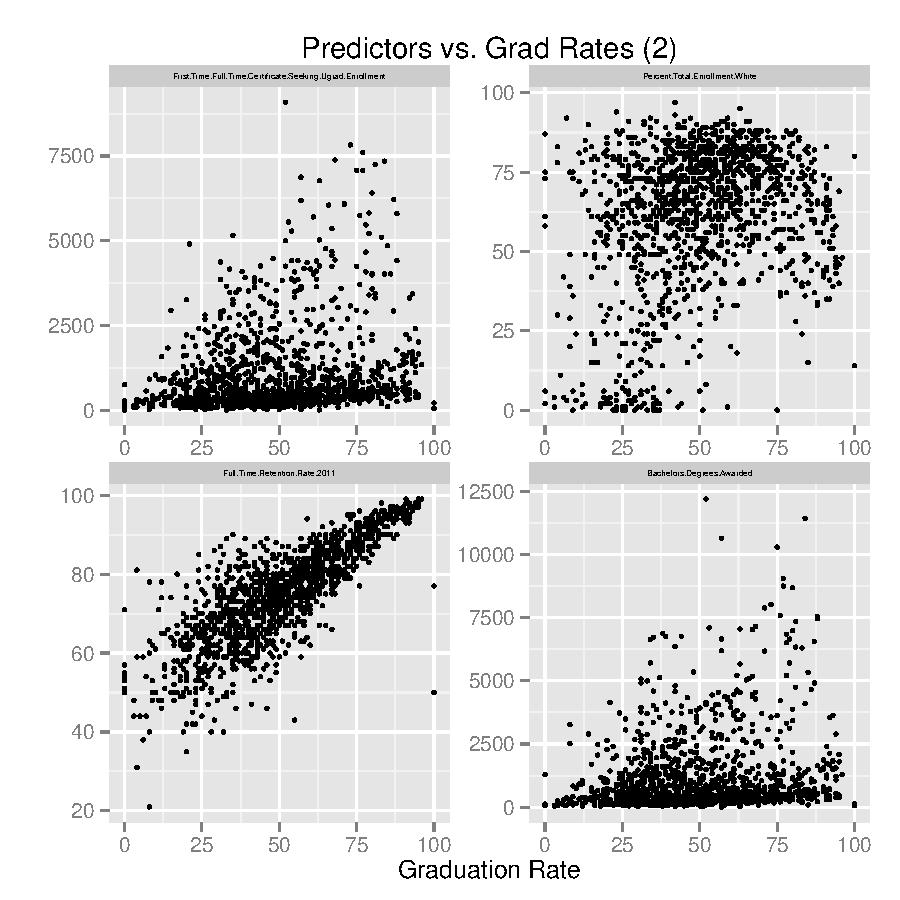
\includegraphics{Fig-scatter2}

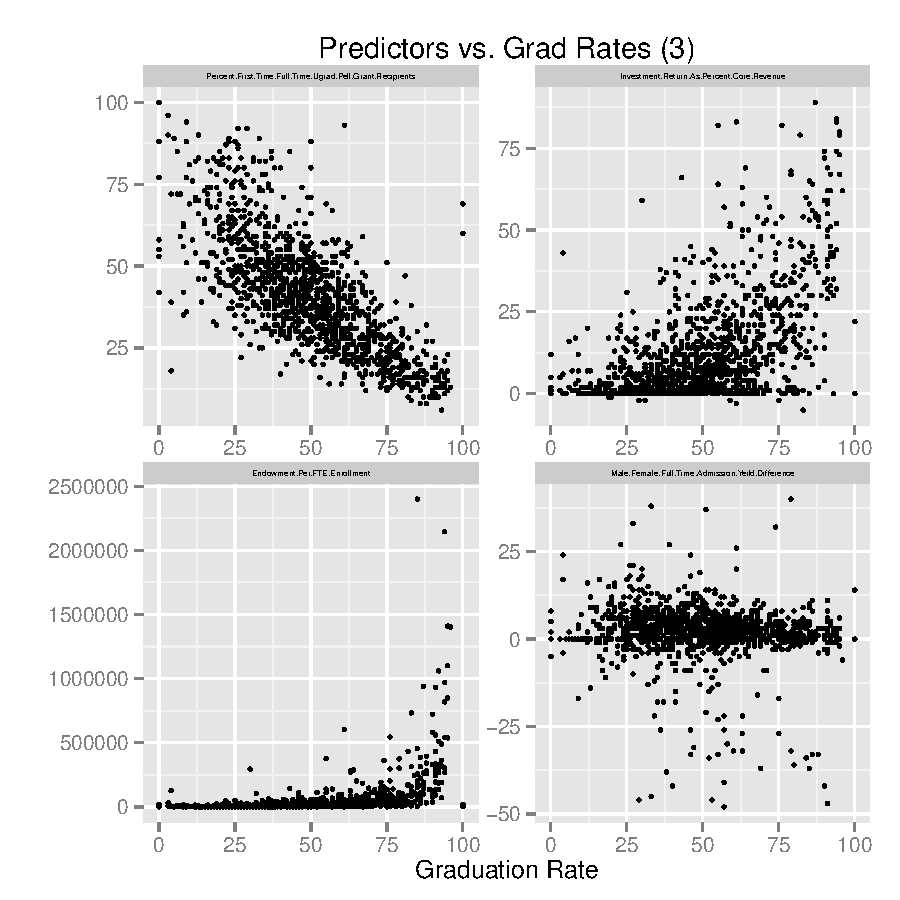
\includegraphics{Fig-scatter3}

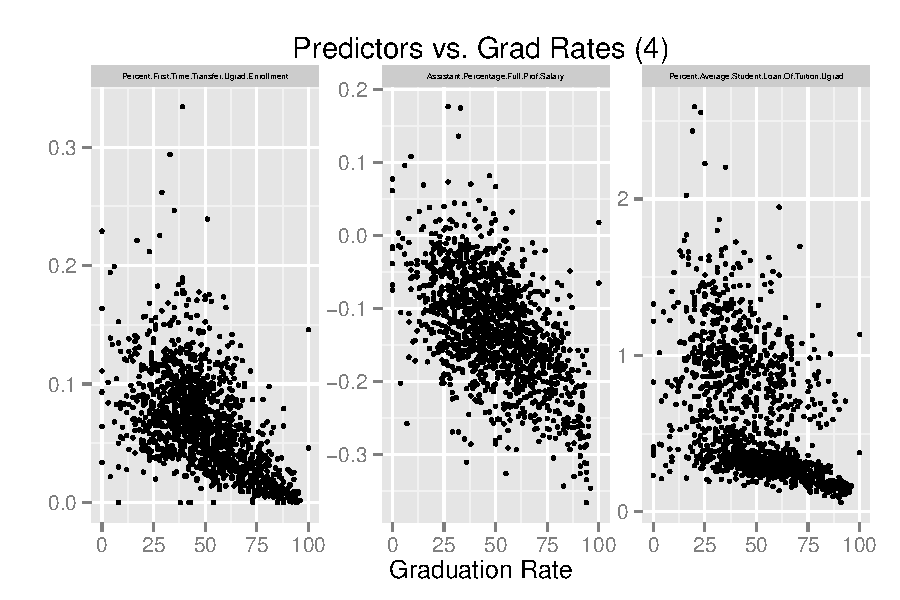
\includegraphics{Fig-scatter4}

\FloatBarrier

It is clear from this excercise that our full model has several serious problems. There are two pairs of variables that are very co-linear and appear to contain almost the same information. "Tuition.Fees.2009.2010" and "Tuition.Fees.2010.2011" as well as "First.Time.Certificate.Seeking.Ugrad.Enrollment" and "First.Time.Full.Time.Certificate.Seeking.Ugrad.Enrollment" are providing almost the same information to the model. This can be confirmed by computing the variance inflation factors for all the variables in the full model. Clearly one variable of each pair should be removed from the model as the VIF value for each component of each pair well above the average VIF of $72.184$.

It is also clear from this table that "Undergraduate.Enrollment" and "Bachelor.Degrees.Awarded" are also causing co-linearity issues, though the issues are not as severe as with the other two pairs of predictors. One would suspect that an institution with a large undergraduate enrollment would also have a large number of bachelor degrees awarded. One of these pair should likely be removed as well.

% latex table generated in R 3.0.2 by xtable 1.7-1 package
% Thu Dec 19 11:05:36 2013
\begin{table}[ht]
\centering
\begin{tabular}{rlr}
  \hline
 & Variable & VIF \\ 
  \hline
1 & Tuition.Fees.2009.2010 & 604.98 \\ 
  2 & Tuition.Fees.2010.2011 & 605.49 \\ 
  3 & Mid.East & 1.13 \\ 
  4 & Distant.Degree.of.Urbanization & 1.04 \\ 
  5 & UgradProfile.FullTime.MoreSelective.HighTransfer & 1.66 \\ 
  6 & UgradProfile.FullTime.MoreSelective.LowTransfer & 3.77 \\ 
  7 & UgradProfile.FullTime.Selective.HighTransfer & 1.73 \\ 
  8 & UgradProfile.FullTime.Selective.LowTransfer & 2.09 \\ 
  9 & UgradProfile.Medium.FullTime.Selective.Inclusive & 1.25 \\ 
  10 & SizeSetting.Large.FourYear.NotResidential & 2.04 \\ 
  11 & SizeSetting.Medium.FourYear.NotResidential & 1.39 \\ 
  12 & SizeSetting.Small.FourYear.NotResidential & 1.22 \\ 
  13 & SizeSetting.Small.FourYear.Residential & 1.23 \\ 
  14 & SizeSetting.VSmall.FourYear.NotResidential & 1.10 \\ 
  15 & Undergraduate.Enrollment & 43.08 \\ 
  16 & First.Time.Certificate.Seeking.Ugrad.Enrollment & 337.65 \\ 
  17 & First.Time.Full.Time.Certificate.Seeking.Ugrad.Enrollment & 292.15 \\ 
  18 & Percent.Total.Enrollment.White & 1.75 \\ 
  19 & Full.Time.Retention.Rate.2011 & 3.26 \\ 
  20 & Bachelors.Degrees.Awarded & 23.94 \\ 
  21 & Percent.First.Time.Full.Time.Ugrad.Pell.Grant.Recipients & 3.66 \\ 
  22 & Investment.Return.As.Percent.Core.Revenue & 2.74 \\ 
  23 & Endowment.Per.FTE.Enrollment & 1.77 \\ 
  24 & Male.Female.Full.Time.Admission.Yeild.Difference & 1.06 \\ 
  25 & Percent.First.Time.Transfer.Ugrad.Enrollment & 2.03 \\ 
  26 & Assistant.Percentage.Full.Prof.Salary & 1.61 \\ 
  27 & Percent.Average.Student.Loan.Of.Tuition.Ugrad & 4.15 \\ 
   \hline
\end{tabular}
\caption{Variance Inflation Factor Table - Full Model} 
\end{table}
\FloatBarrier

Another obvious correction would be to include an indicator variable for public institutions back into the model. The scatter plot panel with tuition on the y axis and graduation rate on the x axis is just the same as our motivating scatter plot which compares the same two variables. There is an interaction between tuition and an institution's identity as public or private that can be evidenced graphically. We should model this relationship with the addition of an interaction term.

One more obvious correction would be to add a variable transformations for endowment per FTE. A scatter plot indicates a diminishing relationship between this variable and graduation rates. An appropriate transform for endowment per FTE appears to be a log transformation.

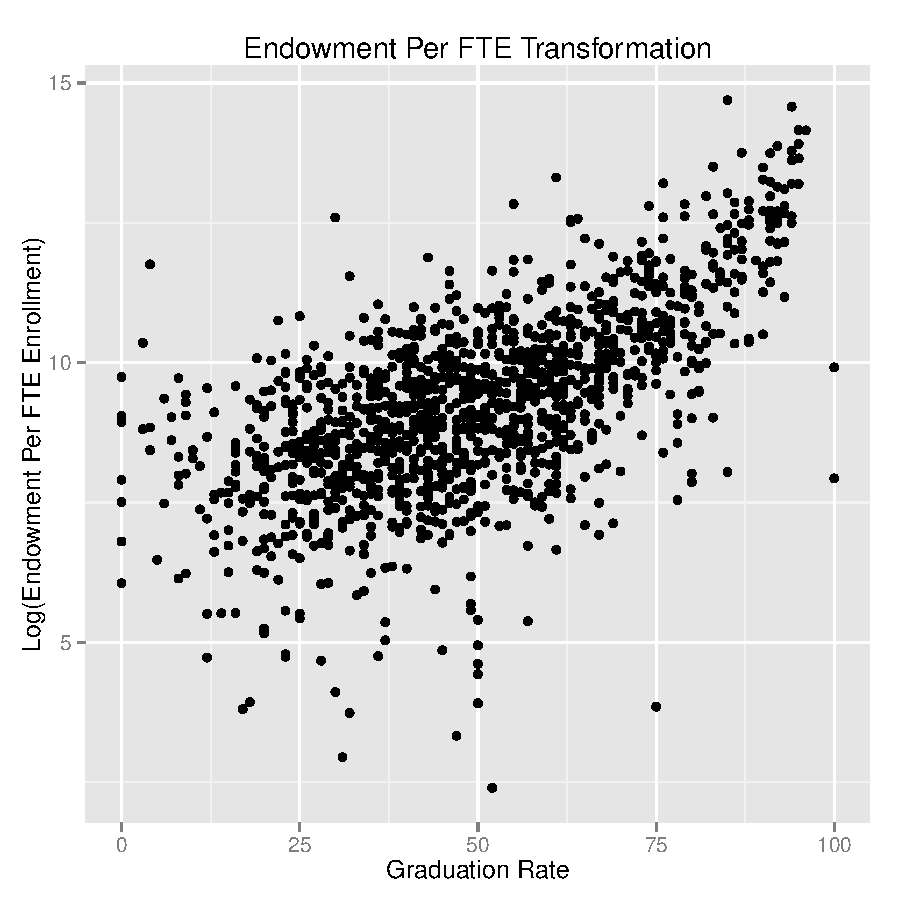
\includegraphics{Fig-transforms}

\FloatBarrier

Before making these corrections though, we have one larger problem. There are several indicators that the residuals are not normally distributed, likely due to outliers. A QQ plot of the residuals suggests that they are distributed with heavy tails. We should attempt to correct this by removing outliers.

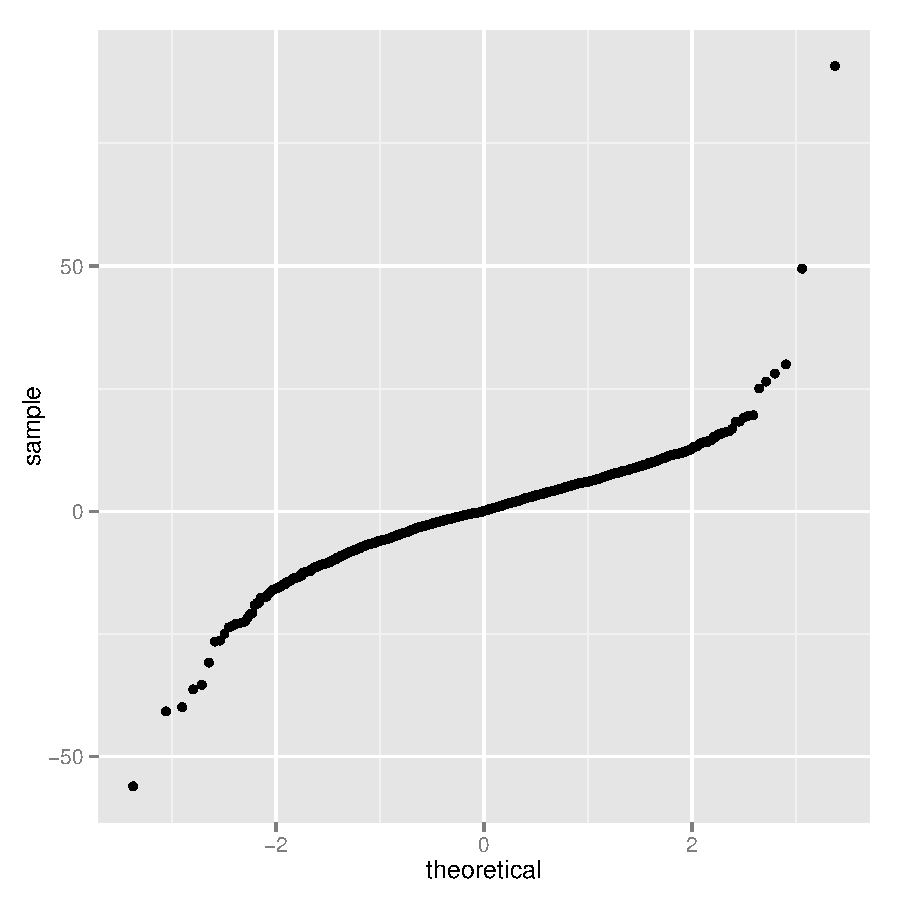
\includegraphics{Fig-qqplot}

\FloatBarrier

\subsection{Outlier Removal}

A histogram of the studentized deleted residuals would suggest that we have several outliers. After calculating the bonferroni critical value for outliers, we can assume that the following observations for five year graduation rate should be removed from the data set. Note that I have set the $\alpha$ level at $\alpha = 0.10$ for the Bonferroni test.

$$ H_0 \text{: Observation Is Not an Outlier in Response} $$
$$ H_a \text{: Observation Is an Outlier in Response} $$
$$ \text{If }t^* > t(1-\frac{\alpha}{2702},1323) = 3.976 \text{ Reject }H_0 $$

Using this test, we remove the observations in table that follows.

\begin{Schunk}
\begin{Sinput}
> library(MASS)
> # find the studentized residuals
> stud.del.res <- studres(grfull)
> # plot a histogram of them
> qplot(stud.del.res,
+       xlab="Studentized Deleted Residuals",
+       binwidth=0.05)
> # set alpha
> alpha <- 0.1
> # calculate the critical value
> ct <- qt(1-alpha/(2*length(stud.del.res)),
+          length(stud.del.res) - length(grfull$coefficients))
> # find the outliers
> groutliers <- which(abs(stud.del.res) > ct)
> print(xtable(data.frame(Institutions = rownames(GradRate)[which(abs(stud.del.res) > ct)]),
+              caption="Observations Removeed Due to Outlying Responses"))
\end{Sinput}
% latex table generated in R 3.0.2 by xtable 1.7-1 package
% Thu Dec 19 11:05:38 2013
\begin{table}[ht]
\centering
\begin{tabular}{rl}
  \hline
 & Institutions \\ 
  \hline
1 & Arizona Christian University : Arizona \\ 
  2 & Holy Cross College : Indiana \\ 
  3 & Franklin Pierce University : New Hampshire \\ 
  4 & Rivier University : New Hampshire \\ 
  5 & Northern New Mexico College : New Mexico \\ 
  6 & Northwest Christian University : Oregon \\ 
  7 & Gwynedd Mercy College : Pennsylvania \\ 
  8 & Hampden-Sydney College : Virginia \\ 
   \hline
\end{tabular}
\caption{Observations Removeed Due to Outlying Responses} 
\end{table}\end{Schunk}
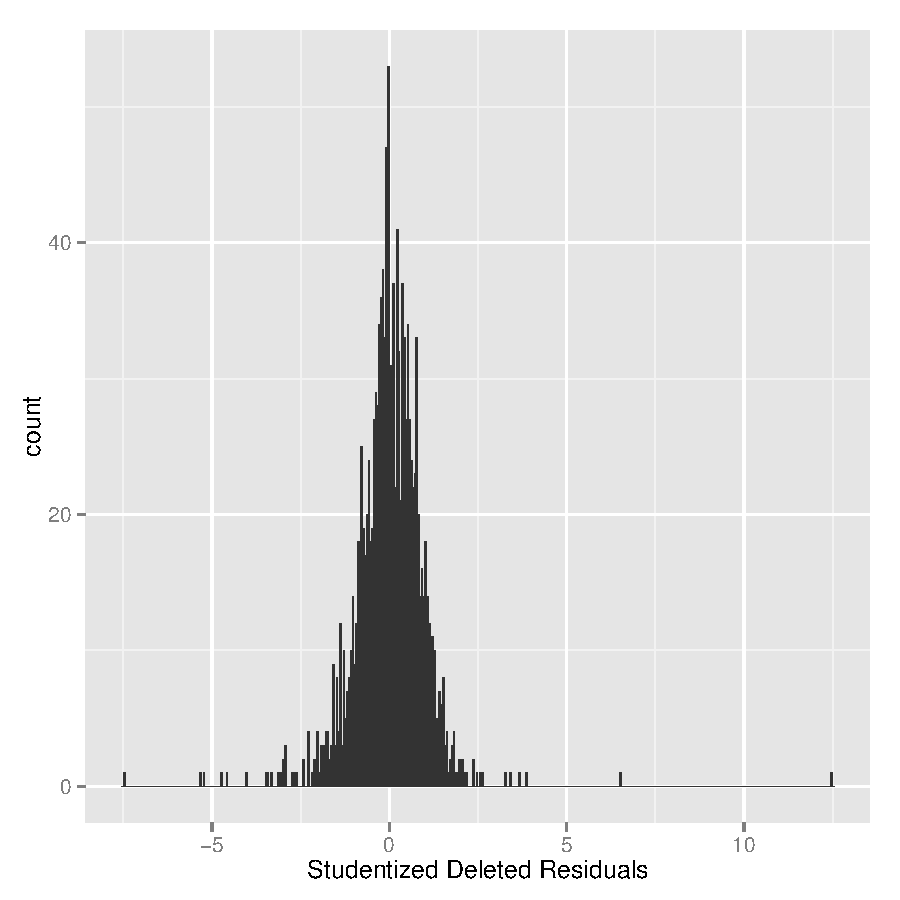
\includegraphics{Fig-residuals}

\FloatBarrier

The predictor variables also have outliers. We use the hat matrix to find them. A table of those removed follows.

\begin{Schunk}
\begin{Sinput}
> # get the diagonal of the hat matrix
> diagonal <- lm.influence(grfull)$hat
> # define the threshold
> threshold <- 2*(length(grfull$coefficients) - 1)/
+   length(grfull$model$Five.Year.Bachelors.Graduation.Rate)
> # find the outliers
> xoutliers <- which(diagonal > threshold)
> print(xtable(data.frame(Institutions = rownames(GradRate)[xoutliers[1:52]],
+                         `Institutions   continued` = rownames(GradRate)[xoutliers[53:104]],
+                         row.names=NULL),
+              caption="Observations Removed Due to Outlying Predictors"))
\end{Sinput}
% latex table generated in R 3.0.2 by xtable 1.7-1 package
% Thu Dec 19 11:05:38 2013
\begin{table}[ht]
\centering
\begin{tabular}{rll}
  \hline
 & Institutions & Institutions...continued \\ 
  \hline
1 & The University of Alabama : Alabama & University of Missouri-St Louis : Missouri \\ 
  2 & Troy University : Alabama & William Jewell College : Missouri \\ 
  3 & University of Alaska Anchorage : Alaska & Bellevue University : Nebraska \\ 
  4 & Arizona State University : Arizona & Peru State College : Nebraska \\ 
  5 & University of Arizona : Arizona & College of Saint Mary : Nebraska \\ 
  6 & Northern Arizona University : Arizona & University of New Hampshire at Manchester : New Hampshire \\ 
  7 & Central Baptist College : Arkansas & Princeton University : New Jersey \\ 
  8 & California Institute of Technology : California & Metropolitan College of New York : New York \\ 
  9 & University of California-Berkeley : California & Cooper Union for the Advancement of Science and Art : New York \\ 
  10 & University of California-Irvine : California & CUNY New York City College of Technology : New York \\ 
  11 & University of California-Los Angeles : California & Morrisville State College : New York \\ 
  12 & University of California-San Diego : California & SUNY Empire State College : New York \\ 
  13 & National University : California & Wells College : New York \\ 
  14 & Pomona College : California & Lees-McRae College : North Carolina \\ 
  15 & San Diego State University : California & William Peace University : North Carolina \\ 
  16 & Thomas Aquinas College : California & Salem College : North Carolina \\ 
  17 & Metropolitan State University of Denver : Colorado & University of Akron Main Campus : Ohio \\ 
  18 & Naropa University : Colorado & Hiram College : Ohio \\ 
  19 & Yale University : Connecticut & Kenyon College : Ohio \\ 
  20 & Trinity Washington University : District of Columbia & Ohio State University-Main Campus : Ohio \\ 
  21 & University of Central Florida : Florida & University of Rio Grande : Ohio \\ 
  22 & Florida Atlantic University : Florida & Tiffin University : Ohio \\ 
  23 & Florida State University : Florida & Langston University : Oklahoma \\ 
  24 & University of Florida : Florida & Oklahoma Panhandle State University : Oklahoma \\ 
  25 & University of South Florida-Main Campus : Florida & Portland State University : Oregon \\ 
  26 & Brewton-Parker College : Georgia & Bryn Athyn College of the New Church : Pennsylvania \\ 
  27 & Macon State College : Georgia & Pennsylvania State University-Main Campus : Pennsylvania \\ 
  28 & Thomas University : Georgia & Providence College : Rhode Island \\ 
  29 & Calumet College of Saint Joseph : Indiana & Erskine College : South Carolina \\ 
  30 & Saint Mary-of-the-Woods College : Indiana & University of South Carolina-Beaufort : South Carolina \\ 
  31 & Southwestern College : Kansas & Presentation College : South Dakota \\ 
  32 & Berea College : Kentucky & Aquinas College : Tennessee \\ 
  33 & Mid-Continent University : Kentucky & Bethel University : Tennessee \\ 
  34 & Midway College : Kentucky & Le Moyne-Owen College : Tennessee \\ 
  35 & Saint Catharine College : Kentucky & Jarvis Christian College : Texas \\ 
  36 & Grambling State University : Louisiana & The University of Texas at Brownsville : Texas \\ 
  37 & University of Maine at Fort Kent : Maine & Texas A \& M University-College Station : Texas \\ 
  38 & University of Maine at Presque Isle : Maine & The University of Texas at Austin : Texas \\ 
  39 & Saint Joseph's College of Maine : Maine & Utah Valley University : Utah \\ 
  40 & University of Maryland-University College : Maryland & Weber State University : Utah \\ 
  41 & University of Maryland-College Park : Maryland & Hampden-Sydney College : Virginia \\ 
  42 & St Mary's College of Maryland : Maryland & Liberty University : Virginia \\ 
  43 & Cambridge College : Massachusetts & Virginia Military Institute : Virginia \\ 
  44 & Harvard University : Massachusetts & Heritage University : Washington \\ 
  45 & Cornerstone University : Michigan & University of Washington-Seattle Campus : Washington \\ 
  46 & Rochester College : Michigan & West Virginia University at Parkersburg : West Virginia \\ 
  47 & University of Michigan-Ann Arbor : Michigan & Alverno College : Wisconsin \\ 
  48 & Michigan State University : Michigan & Silver Lake College of the Holy Family : Wisconsin \\ 
  49 & Finlandia University : Michigan & Stanford University : California \\ 
  50 & Alcorn State University : Mississippi & Soka University of America : California \\ 
  51 & Blue Mountain College : Mississippi & Trine University-Regional/Non-Traditional Campuses : Indiana \\ 
  52 & Columbia College : Missouri & University of South Florida-St. Petersburg Campus : Florida \\ 
   \hline
\end{tabular}
\caption{Observations Removed Due to Outlying Predictors} 
\end{table}\end{Schunk}

\FloatBarrier

Removing outliers in both the response and predictor variables from our full model, the residuals appear much closer to being normally distributed.


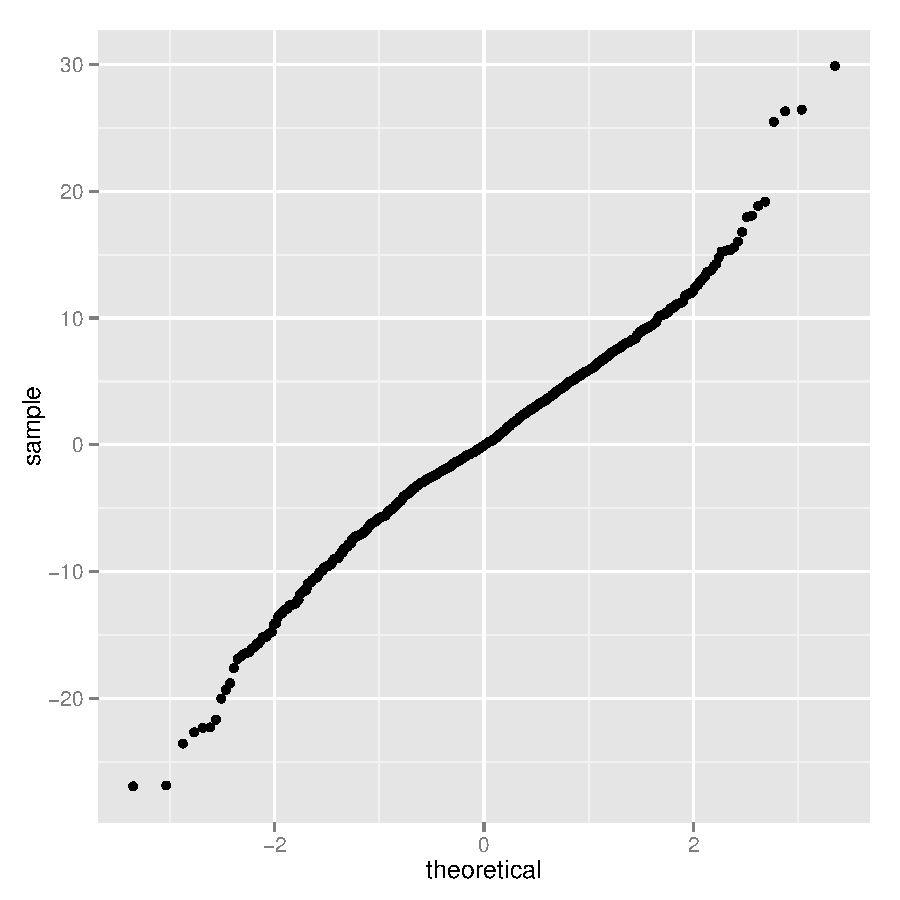
\includegraphics{Fig-qqplotnoouts}


\FloatBarrier

\subsection{Model Refinement}

Now that we have identified outliers in the data, we can estimate the model, incorporating the transformation to endowment per FTE and the interaction of tuition and fees with an institution's status as public or private. Note that the variable "SizeSetting.VSmall.FourYear.NotResidential" has also been removed from this model due to outlier removal. All institutions with this characteristic have been dropped from the model. A model summary table follows:

% latex table generated in R 3.0.2 by xtable 1.7-1 package
% Thu Dec 19 11:05:39 2013
\begin{table}[ht]
\centering
\begin{tabular}{rrrrr}
  \hline
 & Estimate & Std. Error & t value & Pr($>$$|$t$|$) \\ 
  \hline
(Intercept) & -14.0043 & 4.6743 & -3.00 & 0.0028 \\ 
  Tuition.Fees.2010.2011 & 0.0011 & 0.0002 & 5.07 & 0.0000 \\ 
  Mid.East & 2.1592 & 0.5212 & 4.14 & 0.0000 \\ 
  Distant.Degree.of.Urbanization & -5.2771 & 1.9233 & -2.74 & 0.0062 \\ 
  UgradProfile.FullTime.MoreSelective.HighTransfer & 3.6546 & 1.1782 & 3.10 & 0.0020 \\ 
  UgradProfile.FullTime.MoreSelective.LowTransfer & 5.2423 & 0.9752 & 5.38 & 0.0000 \\ 
  UgradProfile.FullTime.Selective.HighTransfer & 1.1431 & 0.6291 & 1.82 & 0.0695 \\ 
  UgradProfile.FullTime.Selective.LowTransfer & 2.2058 & 0.7046 & 3.13 & 0.0018 \\ 
  UgradProfile.Medium.FullTime.Selective.Inclusive & -3.0169 & 0.8246 & -3.66 & 0.0003 \\ 
  SizeSetting.Large.FourYear.NotResidential & -6.4665 & 1.1246 & -5.75 & 0.0000 \\ 
  SizeSetting.Medium.FourYear.NotResidential & -6.7317 & 0.8767 & -7.68 & 0.0000 \\ 
  SizeSetting.Small.FourYear.NotResidential & -5.7885 & 0.9151 & -6.33 & 0.0000 \\ 
  SizeSetting.Small.FourYear.Residential & -2.3676 & 0.6737 & -3.51 & 0.0005 \\ 
  Undergraduate.Enrollment & -0.0004 & 0.0001 & -2.63 & 0.0086 \\ 
  First.Time.Full.Time.Certificate.Seeking.Ugrad.Enrollment & 0.0028 & 0.0008 & 3.65 & 0.0003 \\ 
  Percent.Total.Enrollment.White & 0.0665 & 0.0117 & 5.70 & 0.0000 \\ 
  Full.Time.Retention.Rate.2011 & 0.6633 & 0.0297 & 22.36 & 0.0000 \\ 
  Percent.First.Time.Full.Time.Ugrad.Pell.Grant.Recipients & -0.1642 & 0.0227 & -7.23 & 0.0000 \\ 
  Investment.Return.As.Percent.Core.Revenue & 0.0712 & 0.0227 & 3.14 & 0.0018 \\ 
  Male.Female.Full.Time.Admission.Yeild.Difference & -0.1360 & 0.0274 & -4.97 & 0.0000 \\ 
  Percent.First.Time.Transfer.Ugrad.Enrollment & -2.1561 & 7.1037 & -0.30 & 0.7616 \\ 
  Assistant.Percentage.Full.Prof.Salary & -11.7636 & 3.3780 & -3.48 & 0.0005 \\ 
  Percent.Average.Student.Loan.Of.Tuition.Ugrad & -0.9725 & 1.5585 & -0.62 & 0.5328 \\ 
  Private & 6.2954 & 2.0761 & 3.03 & 0.0025 \\ 
  I(log(Endowment.Per.FTE.Enrollment)) & 0.2719 & 0.2257 & 1.20 & 0.2286 \\ 
  Tuition.Fees.2010.2011:Private & -0.0008 & 0.0002 & -3.88 & 0.0001 \\ 
   \hline
\end{tabular}
\caption{F = 357.8953 (n = 1351 on 1214 degrees of freedom)} 
\end{table}
\FloatBarrier

Some coefficients have lost the individual significance of their coefficients. Scaling of the number of first time certificate seeking undergrads aids it's significance, but others are not aided. It may be necessary to remove them from the model. Additionally, computing the VIF statistic again shows that the tuition and fees interaction with public or private status, as well as undergraduate enrollment and first time certificate seeking undergrad enrollment cause multico-linearity issues in this model. Centering only appears to make the interaction term's contribution to the model's co-linearity issues greater according to the VIF statistic, so we will live with it in its current form. We will now test if we can remove the first time certificate seeking undergrad enrollment variable, as it would appear not to have an individually significant coefficient.

$$ H_0 \text{: } \beta{}_iFirst.Time.Full.Time.Certificate.Seeking.Ugrad.Enrollment = 0 $$
$$ H_a \text{: } \beta{}_iFirst.Time.Full.Time.Certificate.Seeking.Ugrad.Enrollment \neq 0 $$
$$ \text{If } F^* > F(0.99,1,1214) = 7 \text{ Reject }H_0 $$

\begin{Schunk}
\begin{Sinput}
> # estimate the reduced model without First.Time.Full.Time.Certificate.Seeking.Ugrad.Enrollment
> grred.r <- lm(Five.Year.Bachelors.Graduation.Rate~. 
+               + Tuition.Fees.2010.2011*Private 
+               + I(log(Endowment.Per.FTE.Enrollment))
+               - Endowment.Per.FTE.Enrollment
+               - First.Time.Full.Time.Certificate.Seeking.Ugrad.Enrollment,
+               data=GradRate.m)
> grred.rsum <- summary(grred.r)
> # calculate the F statistic
> F_star <- ((deviance(grred.r) - deviance(grred)) /
+              ((length(grred$model$Five.Year.Bachelors.Graduation.Rate)
+                - grred.rsum$df[1]) -
+                 (length(grred$model$Five.Year.Bachelors.Graduation.Rate)
+                  - grredsum$df[1]))) /
+   (deviance(grred)/length(grred$model$Five.Year.Bachelors.Graduation.Rate)
+    - grredsum$df[1])
> # also calculate the critical value
> cv <- qf(0.99,1,
+          length(grred$model$Five.Year.Bachelors.Graduation.Rate)
+          -grredsum$df[1])
> # is the test statistic less than the critical value?
> F_star < cv
\end{Sinput}
\begin{Soutput}
[1] FALSE
\end{Soutput}
\end{Schunk}

$F^*$ is greater than the critical value of $6.6558$ so we cannot remove the first time certificate seeking undergrad variable from the model. The next test shows that we can remove all three of the variables endowment per FTE, the percentage that the average student loan is of tuition, and the percent of first time undergrad transfers enrolled.

$$ H_0 \text{: } \beta{}_{i1},\beta{}_{i2},\beta{}_{i3} = 0 $$
$$ H_a \text{: } \beta{}_{i1},\beta{}_{i2},\beta{}_{i3} \neq 0 $$
$$ \text{If } F^* > F(0.99,3,1214) = 3.7978 \text{ Reject }H_0 $$

\begin{Schunk}
\begin{Sinput}
> # estimate the reduced model
> grred.r <- lm(Five.Year.Bachelors.Graduation.Rate~.
+               + Tuition.Fees.2010.2011*Private
+               - Endowment.Per.FTE.Enrollment
+               - Percent.Average.Student.Loan.Of.Tuition.Ugrad
+               - Percent.First.Time.Transfer.Ugrad.Enrollment,
+               data=GradRate.m)
> grred.rsum <- summary(grred.r)
> # calculate the test statistic F_star
> F_star <- ((deviance(grred.r) - deviance(grred)) /
+              ((length(grred$model$Five.Year.Bachelors.Graduation.Rate)
+                - grred.rsum$df[1]) -
+                 (length(grred$model$Five.Year.Bachelors.Graduation.Rate)
+                  - grredsum$df[1]))) /
+   (deviance(grred)/length(grred$model$Five.Year.Bachelors.Graduation.Rate)
+    - grredsum$df[1])
> # calculate the critical value
> cv <- qf(0.99,3,
+          length(grred$model$Five.Year.Bachelors.Graduation.Rate)
+          -grredsum$df[1])
> # is the test statistic less than the critical value?
> F_star < cv
\end{Sinput}
\begin{Soutput}
[1] TRUE
\end{Soutput}
\end{Schunk}

The test statistic $F^*$ is less than the critical value of $3.7978$, so we can safely remove these predictors from the model. 

A summary of the model that results after this final correction follows:

% latex table generated in R 3.0.2 by xtable 1.7-1 package
% Thu Dec 19 11:05:39 2013
\begin{table}[ht]
\centering
\begin{tabular}{rrrrr}
  \hline
 & Estimate & Std. Error & t value & Pr($>$$|$t$|$) \\ 
  \hline
(Intercept) & -13.6815 & 3.1294 & -4.37 & 0.0000 \\ 
  Tuition.Fees.2010.2011 & 0.0012 & 0.0002 & 7.37 & 0.0000 \\ 
  Mid.East & 2.0845 & 0.5163 & 4.04 & 0.0001 \\ 
  Distant.Degree.of.Urbanization & -5.3102 & 1.9202 & -2.77 & 0.0058 \\ 
  UgradProfile.FullTime.MoreSelective.HighTransfer & 3.7998 & 1.1729 & 3.24 & 0.0012 \\ 
  UgradProfile.FullTime.MoreSelective.LowTransfer & 5.3717 & 0.9579 & 5.61 & 0.0000 \\ 
  UgradProfile.FullTime.Selective.HighTransfer & 1.1342 & 0.6281 & 1.81 & 0.0712 \\ 
  UgradProfile.FullTime.Selective.LowTransfer & 2.2826 & 0.6892 & 3.31 & 0.0010 \\ 
  UgradProfile.Medium.FullTime.Selective.Inclusive & -3.0419 & 0.8235 & -3.69 & 0.0002 \\ 
  SizeSetting.Large.FourYear.NotResidential & -6.3740 & 1.1193 & -5.69 & 0.0000 \\ 
  SizeSetting.Medium.FourYear.NotResidential & -6.7326 & 0.8731 & -7.71 & 0.0000 \\ 
  SizeSetting.Small.FourYear.NotResidential & -5.8104 & 0.9092 & -6.39 & 0.0000 \\ 
  SizeSetting.Small.FourYear.Residential & -2.3800 & 0.6709 & -3.55 & 0.0004 \\ 
  Undergraduate.Enrollment & -0.0004 & 0.0001 & -2.86 & 0.0043 \\ 
  First.Time.Full.Time.Certificate.Seeking.Ugrad.Enrollment & 0.0030 & 0.0007 & 4.04 & 0.0001 \\ 
  Percent.Total.Enrollment.White & 0.0674 & 0.0115 & 5.86 & 0.0000 \\ 
  Full.Time.Retention.Rate.2011 & 0.6621 & 0.0296 & 22.37 & 0.0000 \\ 
  Percent.First.Time.Full.Time.Ugrad.Pell.Grant.Recipients & -0.1660 & 0.0225 & -7.38 & 0.0000 \\ 
  Investment.Return.As.Percent.Core.Revenue & 0.0875 & 0.0189 & 4.64 & 0.0000 \\ 
  Male.Female.Full.Time.Admission.Yeild.Difference & -0.1367 & 0.0273 & -5.00 & 0.0000 \\ 
  Assistant.Percentage.Full.Prof.Salary & -12.1969 & 3.3601 & -3.63 & 0.0003 \\ 
  Private & 7.3259 & 1.4588 & 5.02 & 0.0000 \\ 
  Tuition.Fees.2010.2011:Private & -0.0008 & 0.0002 & -5.32 & 0.0000 \\ 
   \hline
\end{tabular}
\caption{F = 406.9198 (n = 1240 on 1217 degrees of freedom)} 
\end{table}
\FloatBarrier

We still have one more model problem to deal with if we are concerned about using our model for inference - heterskedasticity. Not only is it clear from scatter plots of the residuals versus the response and predictor variables, but the model also exhibits heterskedasticity according the Breusch-Pagan test statistic. Just from the plots, it is clear that most of these problems come from enrollment and investment return variables. Notice the cone shape of the residual plot against these predictors. There is much wider variation in the residuals at lower rather than higher levels for these three variables.

% latex table generated in R 3.0.2 by xtable 1.7-1 package
% Thu Dec 19 11:05:39 2013
\begin{table}[ht]
\centering
\begin{tabular}{rrrlr}
  \hline
 & Breusch-Pagan Statistic & Degrees of Freedom & Test & P Value \\ 
  \hline
1 & 68.59 & 22.00 & studentized Breusch-Pagan test & 0.00 \\ 
   \hline
\end{tabular}
\end{table}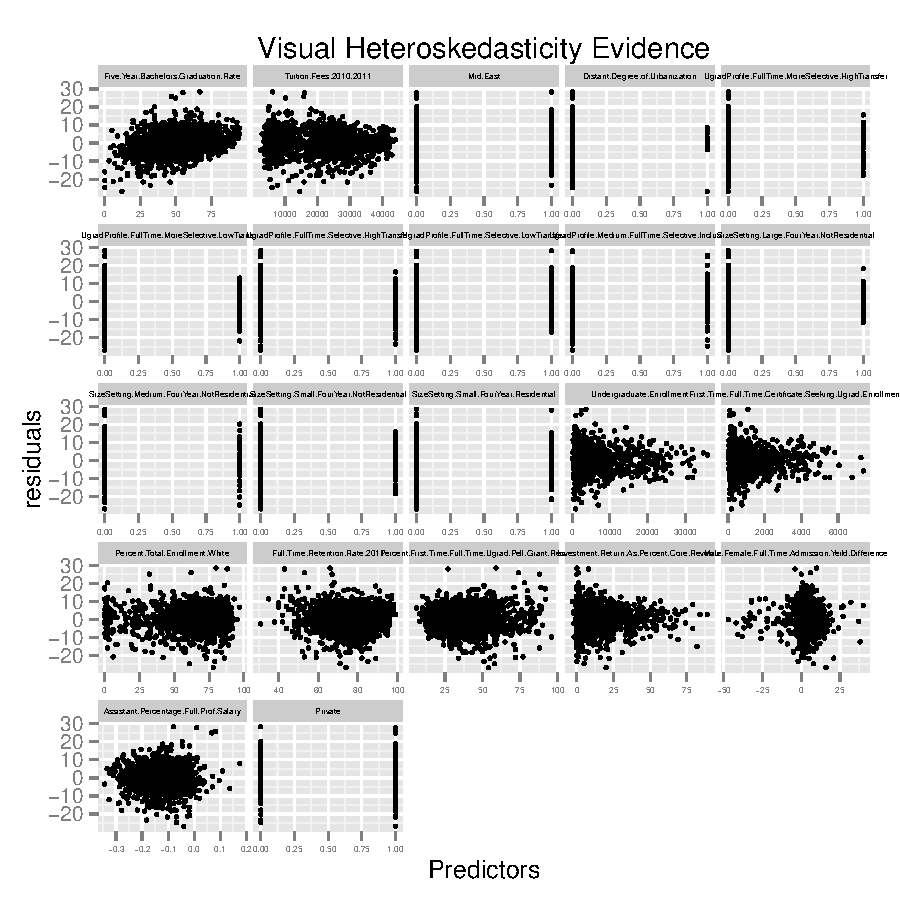
\includegraphics{Fig-bptest}

\FloatBarrier

We can quickly correct for this by producing heteroskedasticity corrected standard errors (HC3 method is used). A table with the new standard errors for each predictor in the model follows. Even after correction of this issue, all but one predictor remains individually significant at at least the $\alpha = 0.1$ level. We will use these corrected standard errors to do prediction and inferencing.

\begin{Schunk}
\begin{Sinput}
> require("sandwich")
> # get a heteroskedasticity-consistent covariance matrix
> grred.r$newse<-vcovHC(grred.r) #uses HC3 method
> # re-do all the t-tests for each coefficient using the new variance-covariance matrix
> print(xtable(as.table(coeftest(grred.r,grred.r$newse,6)),caption="Coefficient Estimation with Robust Standard Errors"))
\end{Sinput}
% latex table generated in R 3.0.2 by xtable 1.7-1 package
% Thu Dec 19 11:05:43 2013
\begin{table}[ht]
\centering
\begin{tabular}{rrrrr}
  \hline
 & Estimate & Std. Error & t value & Pr($>$$|$t$|$) \\ 
  \hline
(Intercept) & -13.68 & 3.71 & -3.69 & 0.01 \\ 
  Tuition.Fees.2010.2011 & 0.00 & 0.00 & 7.45 & 0.00 \\ 
  Mid.East & 2.08 & 0.53 & 3.95 & 0.01 \\ 
  Distant.Degree.of.Urbanization & -5.31 & 2.60 & -2.04 & 0.09 \\ 
  UgradProfile.FullTime.MoreSelective.HighTransfer & 3.80 & 1.24 & 3.06 & 0.02 \\ 
  UgradProfile.FullTime.MoreSelective.LowTransfer & 5.37 & 0.99 & 5.43 & 0.00 \\ 
  UgradProfile.FullTime.Selective.HighTransfer & 1.13 & 0.64 & 1.78 & 0.13 \\ 
  UgradProfile.FullTime.Selective.LowTransfer & 2.28 & 0.73 & 3.11 & 0.02 \\ 
  UgradProfile.Medium.FullTime.Selective.Inclusive & -3.04 & 1.06 & -2.86 & 0.03 \\ 
  SizeSetting.Large.FourYear.NotResidential & -6.37 & 0.99 & -6.44 & 0.00 \\ 
  SizeSetting.Medium.FourYear.NotResidential & -6.73 & 0.92 & -7.35 & 0.00 \\ 
  SizeSetting.Small.FourYear.NotResidential & -5.81 & 1.12 & -5.17 & 0.00 \\ 
  SizeSetting.Small.FourYear.Residential & -2.38 & 0.75 & -3.19 & 0.02 \\ 
  Undergraduate.Enrollment & -0.00 & 0.00 & -3.10 & 0.02 \\ 
  First.Time.Full.Time.Certificate.Seeking.Ugrad.Enrollment & 0.00 & 0.00 & 4.27 & 0.01 \\ 
  Percent.Total.Enrollment.White & 0.07 & 0.01 & 5.28 & 0.00 \\ 
  Full.Time.Retention.Rate.2011 & 0.66 & 0.04 & 17.99 & 0.00 \\ 
  Percent.First.Time.Full.Time.Ugrad.Pell.Grant.Recipients & -0.17 & 0.03 & -6.22 & 0.00 \\ 
  Investment.Return.As.Percent.Core.Revenue & 0.09 & 0.02 & 4.75 & 0.00 \\ 
  Male.Female.Full.Time.Admission.Yeild.Difference & -0.14 & 0.03 & -4.95 & 0.00 \\ 
  Assistant.Percentage.Full.Prof.Salary & -12.20 & 3.56 & -3.43 & 0.01 \\ 
  Private & 7.33 & 1.56 & 4.68 & 0.00 \\ 
  Tuition.Fees.2010.2011:Private & -0.00 & 0.00 & -5.31 & 0.00 \\ 
   \hline
\end{tabular}
\caption{Coefficient Estimation with Robust Standard Errors} 
\end{table}\end{Schunk}

\FloatBarrier

\subsection{Interpretation}

In light of these new standard errors and t statistics, even if we calculate a Bonferroni critical value, which would be $2.0426$ at the $\alpha = 0.05$ level, we reach the conclusion that all but one variable is jointly significant. The variable that doesn't remain is an undergrad profile indicator for institutions that are full time, and selective, but have high rates of transfers in. Because of this, we are able to safely make statements about the full set of predictors. A full discussion follows in the results section.

%-------------------------------------------
\section{Results}
%-------------------------------------------

\subsection{One-Way ANOVA}

They main point of the one-way ANOVA analysis, notwithstanding the issues with the underlying assumptions of the model, is to show that there are true differences between public and private institutions in terms of five year graduation rate. Even despite the problems with the underlying assumptions, we can make this statement with some confidence - the one-way ANOVA on two groups reduces to a t-test, which is highly invariant to departures from normality. There are many potential explanations for this difference. Public schools generally have larger student bodies and they seem to make it difficult for students to graduate in less than five years due to competition for classroom seats. Private colleges also encompass a large majority of the best institutions in the country. These institutions may be contributing to the differences between the two groups. This same conclusion is buttressed by the regression analysis results where, all other things being equal, just being a private institution raises an institution's predicted graduation rate by 7.3 percentage points. This effect is tempered for private schools though. The model also indicates that a \$1,000 increase in tuition and fees is associated with a 1.2 percentage point increase for public schools, but only a 0.4 percent increase for private schools.

\subsection{Two-Way ANOVA}

The two-way ANOVA analysis we should have less confidence in than the one-way version. Unlike the one way version, it does not reduce to a t-test, so we should be wary of the results. If for some reason the results of the analysis were true though, we could note that the relationship between public and private status and graduation rates is not a simple as suggested by the one-way ANOVA analysis. Even at similar levels of selectivity and undergraduate program type, there are still differences in graduation rate as evidenced by a significant F-test for the within group effects for the model. These results are somewhat confirmed by regression analysis. Several of the Carnegie undergraduate program indicators made it into the model, though it appears that only those indicating highly selective institutions when few part-time students were contributory to the model. With the exception of an indicator for selective medium part-time institutions, one would expect the coefficients, as they are for these variables, to be positively correlated with graduation rates. Though no interactions with the private school indicator made it into the model, a prediction for a similarly selective public institution would still be much lower than for a private school because of the primary indicator variable in the model.

\subsection{Regression Analysis}

The regression analysis shows, in a much clearer fashion than the ANOVA analyses, the effect of tuition and fees on graduation rates. After controlling for the selectivity of an institution using Carnegie undergraduate profile variables, for indicators for size and setting that is largely not residential, for degree of urbanization, enrollment, and other variables which we will discuss in brief, tuition and fees appears to have a tempered effect on graduation rates compared to our motivating scatter plot. Every \$1,000 increase in tuition at a public school is associated with a 0.4 percentage increase in graduation rates, while at a public school it is associated with a 1.2 percentage point increase. This seems to say that controlling for other factors, to find a school with good graduation rates, be more willing to pay more for it if it is a public school. This is likely a result of the fact that some of the most prestigious and selective public schools in the country are also the most expensive.

Another interesting effect indicated by the regression model is the relationship between male and female admission yields and graduation rates. After controlling for tuition, selectivity and a host of other factors, as the percentage yield of men gets lower than the percentage yield women, there are huge positive effects on graduation rates (the coefficient is slightly misleading: calculated by subtracting the female admission yeild from male admission yield). This seems to suggest that an institution more acceptable to women than men, is good for graduation rates, but there are likely more factors at play.

An assistant professor's proportion of a full professor's salary also seems to have a significant effect on graduation rates. Oddly enough, as this proportion increases, expected graduation rates decreases.

Two more factors that we found to have interesting associations with graduation rates - retention rates and the percentage of students receiving Pell grants. The positive, and large relationship between retention rates and graduation rates suggests that schools that students stay at are likely to have high graduation rates. While this doesn't lend itself to policy prescriptives since this is largely driven by student transfers, not any inherent educational prescriptive, it would guide an individual college seeker. Places that other students stay at will likely have a high associated five year graduation rate and provide expedient education. 

The relationship between Pell grants and graduation rates is interesting in that it may partial confirm our model. Pell grants are only available for four year periods, so you would expect that institutions where student's have them at a high rate would have to do a better job of affording their student's an education in less than 5 years. In other words, one would expect a negative relationship between Pell grant recipients and graduation rates. As it turns out, our model predicts a negative relationship between these two variables - partially confirming the results.

One last conclusion to be had from the model is that there is a strong negative relationship between large student body size and graduation rates. It appears that big schools are not very efficient educations. This could have some policy prescriptions - simply don't have huge, monolithic educational institutions and graduation rates may rise. Of course, there must be a diminishing effect and a most efficient size, but our model, as currently formulated, does not allow for any analysis of the optimum in the face of those effects.

%-------------------------------------------
\section{Conclusion}
%-------------------------------------------

Graduation rates have many determinants. Most clearly, the selectivity of an institution, the institution's public/private status, and tuition are most closely associated with variation in rates, but other factors are surprisingly related. Though the regression model hints at a few causal mechanisms (may there be something to the male, female admission yield differential), this model is inadequate for addressing the causal mechanism behind graduation rates. One cannot simply assume that an institution's status as a public institution causes it to have a lower graduation rate - rather there may be something about the nature of the students who attend, plus the institution itself that generates a particular graduation rate. More granular data, potentially at the student level, would allow for such an analysis.

%-------------------------------------------
\section{Software References}
%-------------------------------------------

\begin{enumerate}[1)]
\item Achim Zeileis, Torsten Hothorn (2002). Diagnostic Checking in Regression Relationships. R News 2(3), 7-10.
\indent URL: http://CRAN.R-project.org/doc/Rnews/
\item Venables, W. N. \& Ripley, B. D. (2002) Modern Applied Statistics with S. Fourth Edition. Springer, New York. ISBN 0-387-95457-0
\item John Fox and Sanford Weisberg (2011). An {R} Companion to Applied Regression, Second Edition. Thousand Oaks CA: Sage. 
\indent URL: http://socserv.socsci.mcmaster.ca/jfox/Books/Companion
\item David B. Dahl (2013). xtable: Export tables to LaTeX or HTML. R package version 1.7-1. 
\indent http://CRAN.R-project.org/package=xtable
\item Sanford Weisberg (2005). Applied Linear Regression, Third Edition. Hoboken NJ: Wiley. 
\indent URL: http://www.stat.umn.edu/alr
\item Hadley Wickham (2007). Reshaping Data with the reshape Package. Journal of Statistical Software, 21(12), 1-20. 
\indent URL http://www.jstatsoft.org/v21/i12/.
\item H. Wickham. ggplot2: elegant graphics for data analysis. Springer New York, 2009.
\item Thomas Lumley using Fortran code by Alan Miller (2009). leaps: regression subset selection. R package version 2.9. 
\indent http://CRAN.R-project.org/package=leaps
\item Achim Zeileis (2004). Econometric Computing with HC and HAC Covariance Matrix Estimators. Journal of Statistical Software 11(10), 1-17. 
\indent URL http://www.jstatsoft.org/v11/i10/.
\item Yihui Xie (2013). knitr: A general-purpose package for dynamic report generation in R. R package version 1.4.1.
\item Yihui Xie (2013) Dynamic Documents with R and knitr. Chapman and Hall/CRC. ISBN 978-1482203530
\item Yihui Xie (2013) knitr: A Comprehensive Tool for Reproducible Research in R. In Victoria Stodden, Friedrich Leisch and Roger D. Peng, editors, Implementing Reproducible Computational Research. Chapman and Hall/CRC. ISBN 978-1466561595
\item R Core Team (2013). R: A language and environment for statistical computing. R Foundation for Statistical Computing, Vienna, Austria. 
\indent URL http://www.R-project.org/.
\end{enumerate}

\end{document}
